\documentclass[10pt,a4paper]{article}
\usepackage[margin=2.2cm]{geometry}
\usepackage{fontspec}
\usepackage{kotex}
\setmainfont{Apple SD Gothic Neo}
\setsansfont{Apple SD Gothic Neo}
\usepackage{amsmath,amssymb}
\usepackage{graphicx}
\usepackage{caption}
\usepackage[dvipsnames]{xcolor}
\usepackage[colorlinks=true,linkcolor=MidnightBlue,citecolor=MidnightBlue,
            urlcolor=MidnightBlue]{hyperref}
\usepackage{titlesec}
\titleformat{\section}{\large\bfseries}{\thesection}{0.6em}{}
\captionsetup{font=small,labelfont=bf}
\setlength{\parskip}{0.35em}
\setlength{\parindent}{0pt}
\usepackage{mdframed}
\newmdenv[linewidth=0.4pt,linecolor=gray!60,backgroundcolor=gray!5,
          innertopmargin=6pt,innerbottommargin=6pt,skipabove=8pt,skipbelow=8pt]{claimbox}
\newcommand{\claim}[2]{\begin{claimbox}\textbf{주장.} #1\par\smallskip
  \textcolor{gray!70}{\textbf{반증 조건.} #2}\end{claimbox}}

\title{\bfseries 세 문이 다 답했다\\[2pt]
\large 서빙 경로 실물 감사 --- 산문이던 정책이 코드 경로의 규약이 됐다}
\author{월드모델 실험실 · 노트 $855$}
\date{2026-08-09}
\begin{document}\maketitle

\section{한 줄}

$852{\sim}854$ 가 만든 서빙 정책(무정체 기본값 · `만화' 정체 금지 · 이득 지도
라우팅)은 산문이었다 --- 티처 \#$20$ 의 표현으로 ``정책이 설 마루가 없다.''
세 전제를 코드 경로에서 실측했다: \textbf{① 판 배치 무해}(전체 $0.4703$ 대
라벨 $0.4710$ · $\Delta$판 $+0.00065 <$ 씨앗SD --- $849$ 티처 \#$15$ 의 물음
종결) \textbf{② 폴백 우연 안전}(등록 대 미등록의 자루 원점수 해시까지 동일
--- 짝 행렬의 ALL$5$ 선두 정합 덕이며, 조건이 다르면 지뢰는 산다)
\textbf{③ 혼합 배치는 무정체조차 비보존}($322$행 중 $186$ 이동 · $\rho$ 는
$-0.0013$ 소폭 --- 출력층 근접짝 캐스케이드).

\begin{figure}[t]\centering
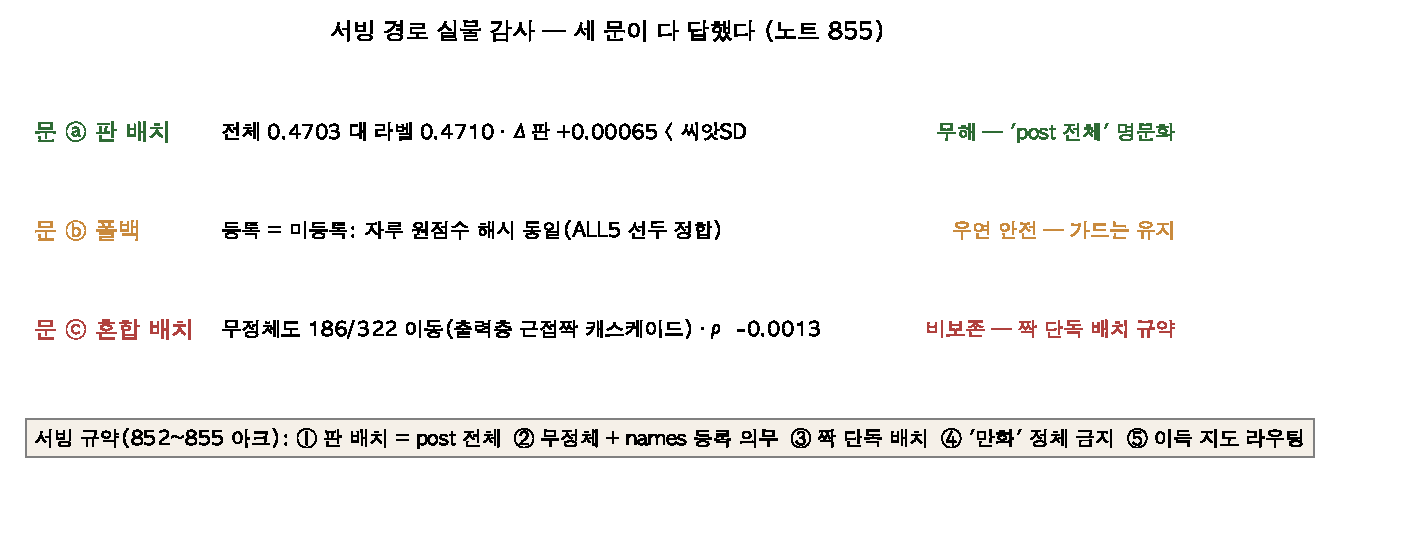
\includegraphics[width=0.97\textwidth]{figs/threedoors.pdf}
\caption{세 문의 판정과 서빙 규약 다섯.}
\end{figure}

\claim{\textbf{서빙 규약 다섯이 확정됐다}: ① 판 채점 배치 $=$ post 전체
② 신규 도메인 $=$ 무정체 $+$ names 명시 등록 의무 ③ 서빙 배치 $=$ 짝 단독
고정(혼합 금지 --- 정확도가 아니라 재현성 문제) ④ `만화' 정체 부여 금지
⑤ 이득 지도 라우팅(KR 는 라벨 $800$건까지 전이 · 앱은 $(20,50]$ 부터 로컬).
남은 실행 주체는 매처 v$1$(들어오는 행이 어느 짝인지 아는 분류기) 하나다.}
{내 코드 독해 예측이 $2/4$ 로 두 번 반증됐다: 폴백 불일치 $80\%$(실제는
우연한 구조 정합) · 무정체 혼합 보존 $75\%$(내가 발견한 출력층 기제를 내가
과소적용). `기제 예측 금지' 규율을 코드 독해 예측에도 확장한다.}

\section{정직}

혼합 대조의 판 행은 만화 · 아이돌 유보뿐(전 조성 미탐색). 폴백 등가는 씨앗
$0$ 의 설계행렬 · 전 자루 기준. 티처 \#$20$ 의 $854$ 정정도 이행: `$11$개
불활성' $\to$ $5$ 정확 불활성 · $6$ 약활성-무해 · $1$ 유해(그리고 귀속은
`만화 원핫'이 아니라 `만화 정체 경로'까지) · 앱 $n^{\dagger} = (20, 50]$ ·
CN 영화 $=$ 만화 동률 최저(기제 후보 하향). GitHub 흐름 $15$회째. 판 $\rho$
$0.4710$ 그대로.

\end{document}
